\label{chap:testing}
This chapter deals with the experiments performed and the results obtained for our framework. The
performance of OpenMP code generated by Polly compared with that of the code generated
by various compilers on various machines. In the first section a simple program
is tested to show that we get similar performance as that of a program having manual OpenMP
annotations. Then in the next section we deal with test cases available in the PolyBench
benchmark.
\section{A simple test case}
The following loop is tested on different machines and the results are shown in the Table ~\ref{table:simple}.
%\begin{verbatim}
{\footnotesize
\begin{lstlisting}
  for (i = 0; i < 1024; i++) {
    for (j = 0; j < 5000000; j++)
      A[i] += j;
  }
\end{lstlisting}
}
%\end{verbatim}
The comparison is made in four different machines with the code compiled with
\begin{itemize}
\item Clang\footnote{\url{http://clang.llvm.org}} which generates only serial code (Serial Execution).
\item Polly with OpenMP enabled which generates necessary OpenMP code automatically (Automatic
      Parallelization).
\item GCC with OpenMP enabled. Here the user have to give the OpenMP pragmas manually (Manual Parallelization).
\end{itemize}
\begin{table}[h]
\begin{center}
{\footnotesize
\begin{tabular}{| l | p{2cm} | p{2cm} | p{2cm} | p{2cm} |}
\hline
& \textbf{Serial Execution} & \textbf{Automatic Parallelization(Polly)} & \textbf{Manual Parallelization(GCC)} \\ \hline
\textbf{Intel Core 2 Duo}(32 Bit OS)& 9.509s & 4.852s & 4.835s \\ \hline
\textbf{Intel Core 2 Duo}(64 Bit OS)& 6.40s  & 3.32s & 3.50s\\ \hline
\textbf{Intel Core i5}(64 Bit OS)   & 6.96s  & 3.78s & 3.75s\\ \hline
\textbf{AMD Engineering Sample(24 Core)}(64 Bit OS)   & 17.039s & 0.757s & 0.796s\\
\hline
\end{tabular}
}
\end{center}
\caption{Performance Comparison}
\label{table:simple}
\end{table}
It can be observed that when OpenMP is enabled in Polly we are getting a performance
almost similar to GCC  with OpenMP pragmas provided by the user manually, which is the expected result. More
speedup is obtained in the 24 Core machine.

\section{PolyBench}
The framework is tested with polyBench 1.0\footnote{\url{http://www-roc.inria.fr/~pouchet/software/polybench/}}
and the results are shown in the next section. PolyBench is a set of computationally intensive programs often
used in the polyhedral community. There are benchmarks from linear algebra, datamining, stencil computation
and solver and manipulation algorithms operating on matrices. On those benchmarks Polly extracts the relevant SCoPs and optimizes them automatically.

\section{Experimental results}
\begin{figure}
\begin{center}
  %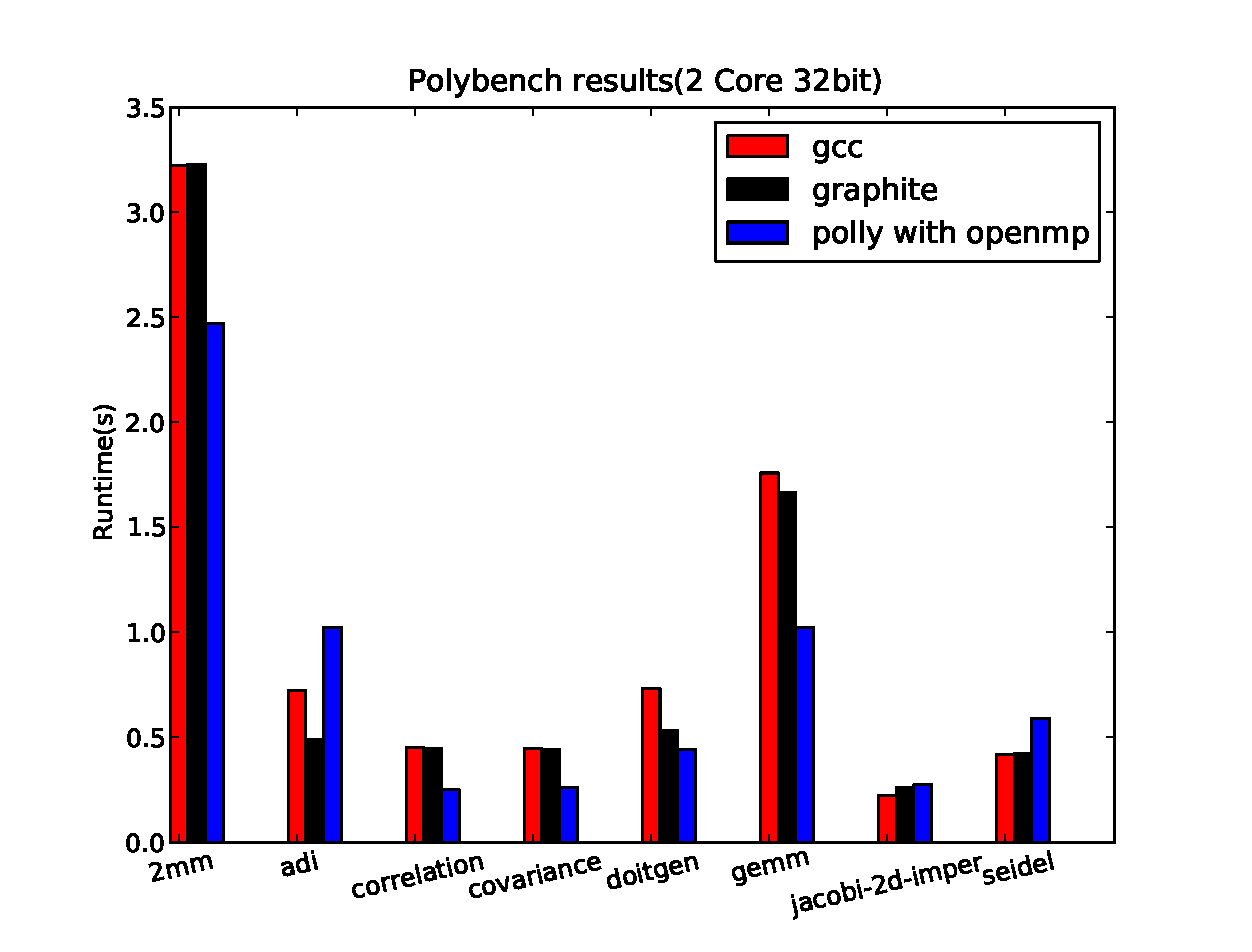
\includegraphics[width=1\textwidth]{images/2core32bit.eps}
  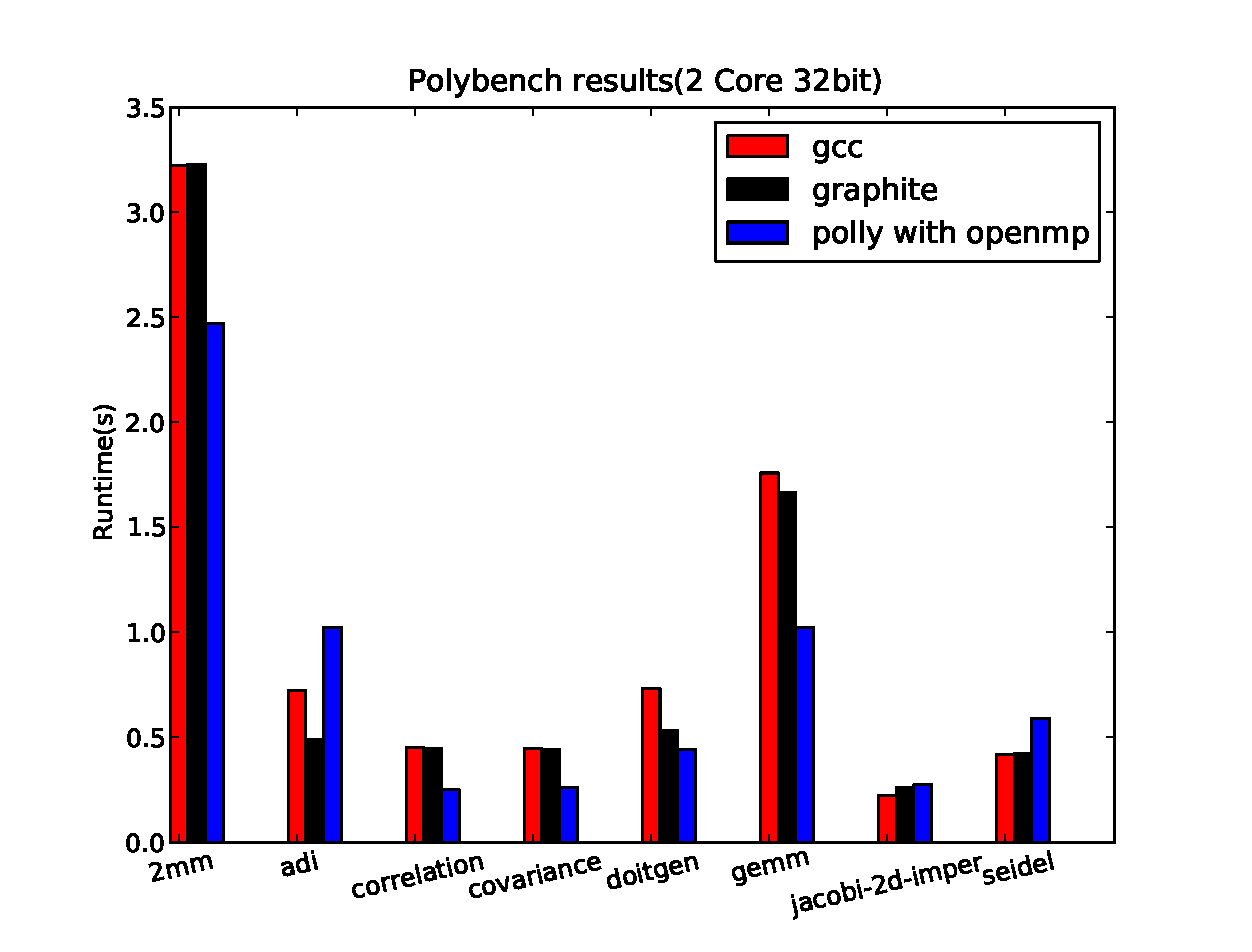
\includegraphics[height=9cm]{images/2core32bit.eps}
  \caption{Performance comparison(2 core 32 bit)}
  \label{fig:2core1}
\end{center}
\end{figure}

\begin{figure}
\begin{center}
  %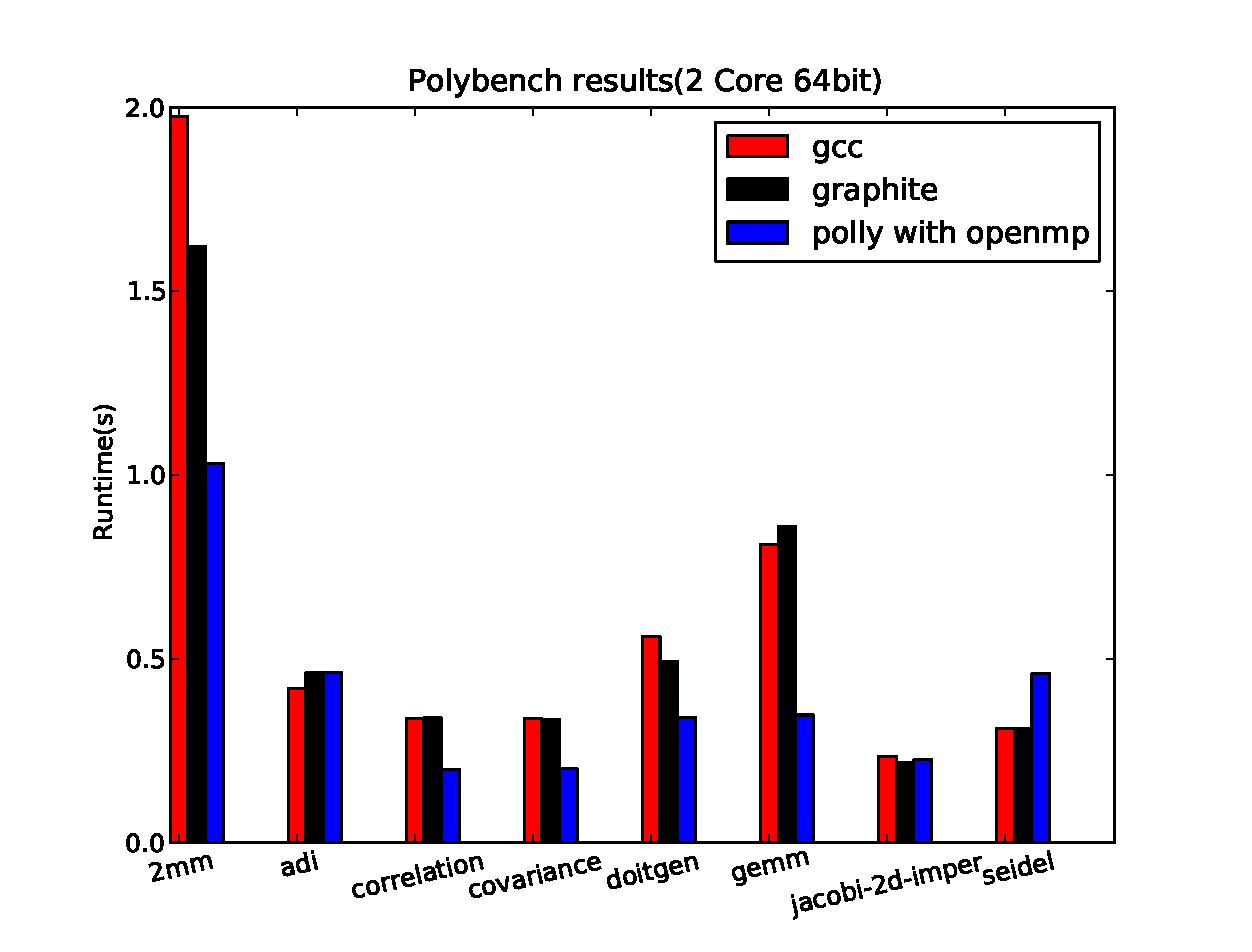
\includegraphics[width=1\textwidth]{images/2core64bit.eps}
  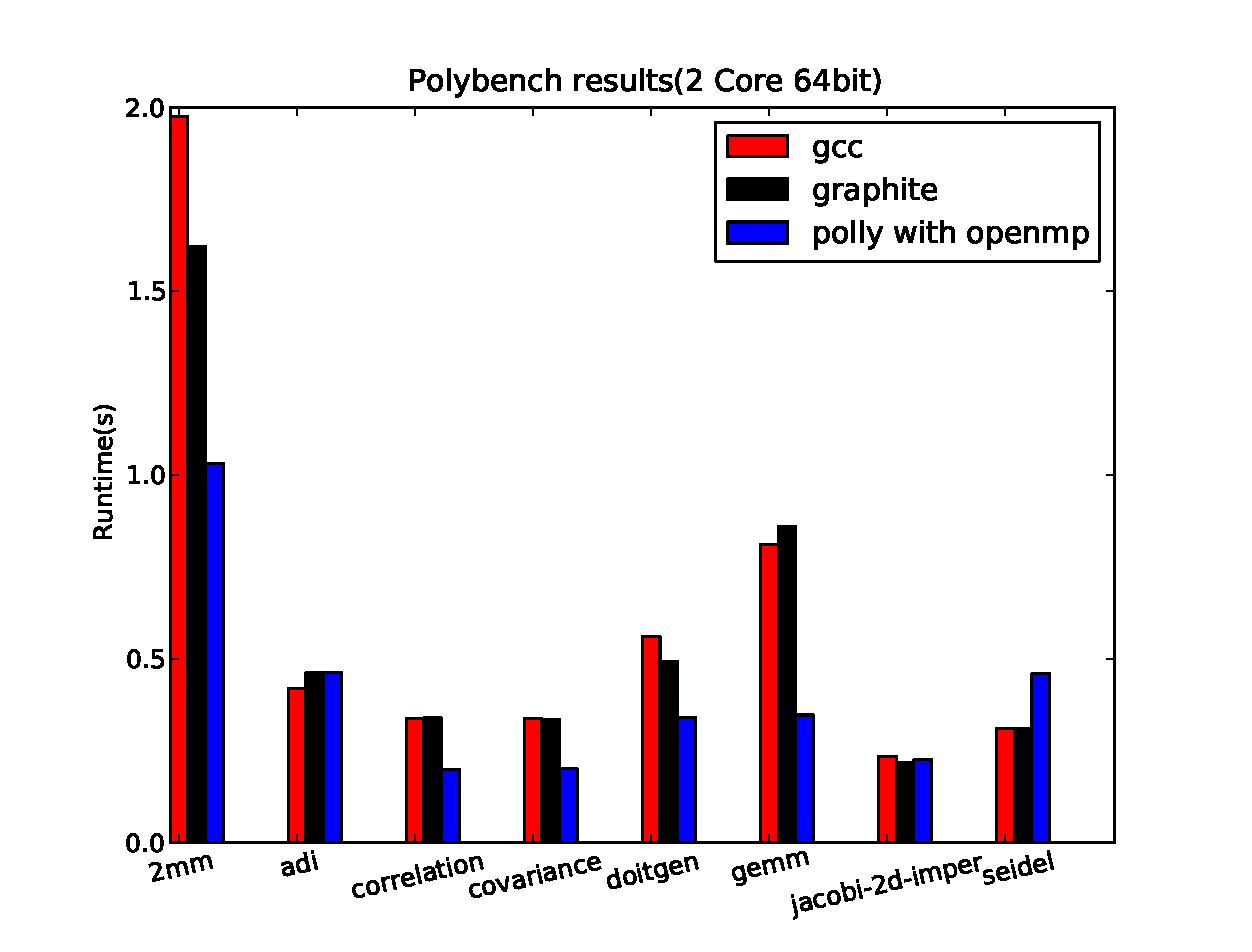
\includegraphics[height=9cm]{images/2core64bit.eps}
  \caption{Performance comparison(2 core 64bit)}
  \label{fig:2core2}
\end{center}
\end{figure}

\begin{figure}
\begin{center}
  %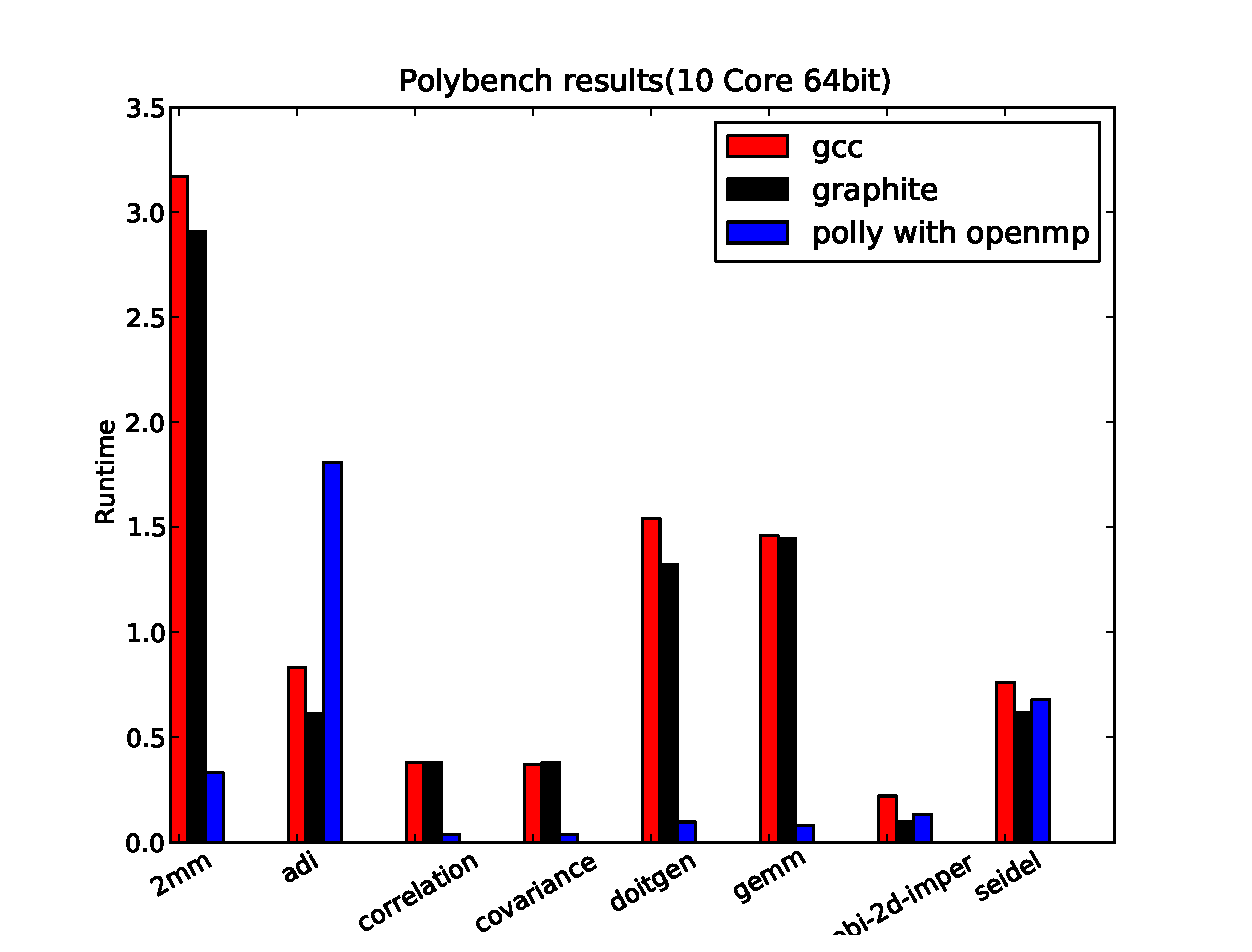
\includegraphics[width=1\textwidth]{images/10core64bit.eps}
  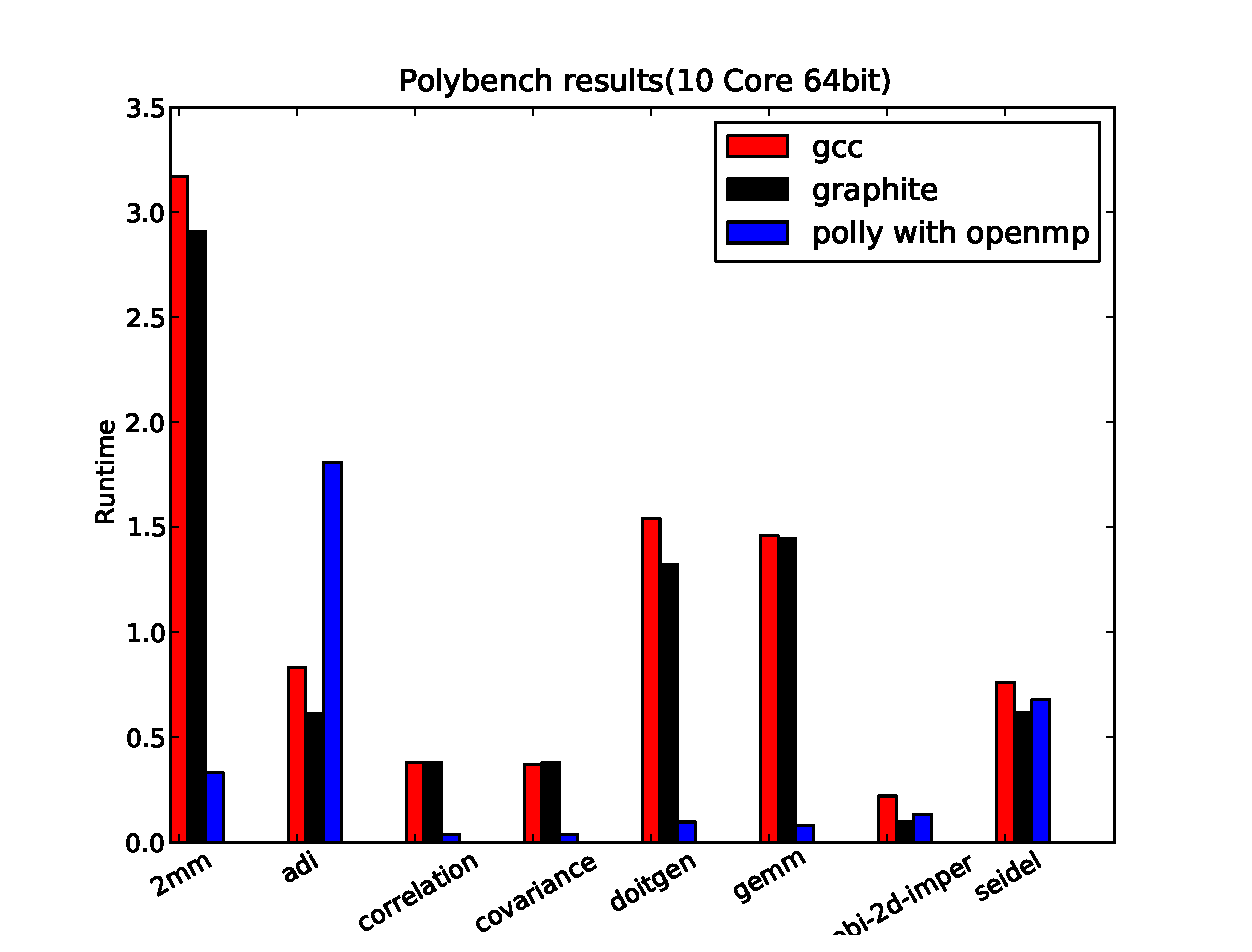
\includegraphics[height=9cm]{images/10core64bit.eps}
  \caption{Performance comparison(10-core 64 bit)}
  \label{fig:10core}
\end{center}
\end{figure}

The OpenMP code generated by Polly is compared with gcc and graphite\cite{TRIFUNOVIC:2010}. With gcc
we make a comparison with serial execution and with graphite we make comparison
with an existing autoparallelization framework, which is also based on polyhedral
model. 
The tests are carried out in 3 different machine with the following configurations

\begin{itemize}
\item Intel Core 2 Duo with 32 Bit OS
\item Intel Core 2 Duo with 64 bit OS
\item 10-Core AMD Engineering Sample with 64 Bit OS
\end{itemize}
The 10-core machine is part of GCC compile farm\footnote{\url{http://gcc.gnu.org/wiki/CompileFarm}}. The GCC Compile farm project maintains
a set of machines of various architectures and provides ssh access to free software developers, GCC and others.
Once the account application  is approved, we get full ssh access to all the farm machines. Then we
are free to install any packages and test our work. The only prerequisite to get access is that
we should be an active contributer for at least one free software project.

The script for testing is given below and the results are shown in the graphs in
Figures ~\ref{fig:2core1}, ~\ref{fig:2core2} and ~\ref{fig:10core}.
{\footnotesize
\begin{lstlisting}
# serial
gcc -I utilities utilities/instrument.c -DPOLYBENCH_TIME   \
                      -DPOLYBENCH_DUMP_ARRAYS -O3 $1 -lm
# Autopar with graphite
n = 4 # n = 2 for 2 core, n = 10 for 10-core
gcc -I utilities utilities/instrument.c -DPOLYBENCH_TIME   \
           -DPOLYBENCH_DUMP_ARRAYS -O3 -floop-interchange  \
           -floop-block -floop-parallelize-all             \
	   -ftree-parallelize-loops=$n $1 -lm
# Autopar with polly OpenMP
pollycc -fpolly -fparallel -I utilities utilities/instrument.c \
              -DPOLYBENCH_TIME -DPOLYBENCH_DUMP_ARRAYS  $1 -lm
\end{lstlisting}
}
While we look into the results it can be observed that Polly with OpenMP support
shows nice performance other than the benchmarks 'adi' and 'seidel'. The reason
for this is, due to dependences, the parallelism detection algorithm available
in Polly is not able to detect the kernel of these testcases as parallel. Consider
the kernel of 'seidel' given below.

{\footnotesize
\begin{lstlisting}
for (t = 0; t <= tsteps - 1; t++)
  for (i = 1; i<= n - 2; i++)
    for (j = 1; j <= n - 2; j++)
      A[i][j] = (A[i-1][j-1] + A[i-1][j] + A[i-1][j+1]
		+ A[i][j-1] + A[i][j] + A[i][j+1]
		+ A[i+1][j-1] + A[i+1][j] + A[i+1][j+1])/9.0;
\end{lstlisting}
}

This has some loop carried dependences due to which Polly fails to detect parallelism. In this case Polly can get help
from PLUTO optimizations. PLUTO can transform the loop in a way that some parallelism can be extracted.
It is observed that OpenMP code is generated in this way. But the result was not improved at least
in case of 'seidel'. It was improved when the OpenMP scheduling policy is changed. The default scheduling
policy set while generating OpenMP code is 'runtime', using which the user can provide
one of the three scheduling algorithms('static', 'guided', 'dynamic'). This can be set
at runtime with the environment variable 'OMP\_SCHEDUlE'. The performance of 'seidel is
improved with 'OMP\_SCHEDULE' set to 'guided' with 'PLUTO'. But for 'adi' even without help from PLUTO, just setting
'OMP\_SCHEDULE' was enough to improve performance. The results are shown in Table ~\ref{table:seidel}

\begin{table}[h]
\begin{center}
{\footnotesize
\begin{tabular}{| l | p{2cm} | p{2cm} | p{2cm} | p{2cm} |}
\hline
& \textbf{Serial Execution} & \textbf{Polly + OpenMP} & \textbf{Polly + PLUTO + OpenMP} \\ \hline
\textbf{2 Core 32 Bit} & 0.417174s & 0.591673s & 0.348909s \\ \hline
\textbf{2 Core 64 Bit} & 0.310160s  &  0.459641s & 0.254605s\\ \hline
\end{tabular}
}
\end{center}
\caption{Performance improvement of seidel}
\label{table:seidel}
\end{table}

Another interesting result observed is when 'seidel is tested in 10-core machine with larger
data size(N=4096). There is significant variations when the OpenMP parameters are tuned to different
values. Optimizations is done with the combination of Polly and PLUTO. The scheduling policy
is set to 'guided' and other parameters(chunk size and number of
OpenMP threads) are varied. The results are show in Table ~\ref{table:seidel:10core}

\begin{table}[h]
\begin{center}
{\footnotesize
\begin{tabular}{| c | p{2cm} | p{2cm} | p{2cm} | p{2cm} |}
\hline
\backslashbox {No of threads}{Chunk size} &                 \textbf{512}  & \textbf{256}  & \textbf{128}  \\ \hline
  \textbf{default} & 12.930170s &  11.254353s   &  37.003882s   \\ \hline
  \textbf{10}      & 15.433336s &  14.657253s   &  14.518356s   \\ \hline
  \textbf{5}       & 14.002886s &  12.283284s   & 14.018281s    \\ \hline
  \textbf{2}       & 16.649145s &  18.778266s   & 18.013177s    \\ \hline
\end{tabular}
}
\end{center}
\caption{Performance of seidel with different OpenMP parameters}
\label{table:seidel:10core}
\end{table}

A sub project for Polly  is already planned to increase  the coverage and performance of Polly, which
will consider various possibilities for improvement. For details refer to Chapter ~\ref{chap:future}.



